\chapterimage{chapter_head_2.pdf} % Chapter heading image

\chapter{\textcolor{blue}{Fundamentos de musicalidade (dança)}}

\begin{definition}[Musicalidade:] 
\index{Musicalidade}
\label{def:Musicalidade}
O Dicionário Online de Português define musicalidade como \cite{diciomusicalidade}:
\begin{itemize}
\item Particularidade, característica ou estado do que é musical.
\item Tendência natural, \textbf{sensibilidade} ou talento para criar ou tocar música.
\item \textbf{Sensibilidade} para contemplar música; \textbf{conhecimento} sobre música.
\item A \textbf{demonstração do talento} musical de uma pessoa.
\end{itemize}
\end{definition}


%% Informação mutua vs Correlação
%% Exemplo dançar em coerencia com a música
%% Eurythmics - Sweet Dreams (Are Made Of This) (Official Video)

%%%%%%%%%%%%%%%%%%%%%%%%%%%%%%%%%%%%%%%%%%%%%%%%%%%%%%%%%%%%%%%%%%%%%%%%%%%%%%%%
%%%%%%%%%%%%%%%%%%%%%%%%%%%%%%%%%%%%%%%%%%%%%%%%%%%%%%%%%%%%%%%%%%%%%%%%%%%%%%%%
\section{Musicalidade, sentir ou entender a música?}
Seguindo a Definição \ref{def:Musicalidade}, podemos inferir como entender a musicalidade na dança.
Esta acontece, quando o dançarino tem um estado de ``sensibilidade'' ou ``conhecimento'' para contemplar ou entender a música,
e assim quando este dança, ``demostrar'' uma coerência entre a música e o que está dançando.

Porem temos um choque de paradigmas, na definição, para atingir um mesmo objetivo que é ser musical.
Podemos \textbf{sentir} ou \textbf{conhecer}; o que é equivalente a dizer que:
\begin{itemize} 
\item podemos saber, por intuição sem entender porquê, ou
\item podemos saber, entendendo mediante o conhecimento adquirido pelo raciocínio e o estudo.\\
\end{itemize}



Neste sentido, para adquirir esta coerência com a música, 
muitos professores indicam que o dançarino deve ``escutar e sentir a música'';
nesse aspecto, argumento que a frase é metaforicamente correta e coincide em parte com a Definição \ref{def:Musicalidade};
porem, pedagogicamente  é pouco favorável para o estudante.
Assim, eu ressaltaria que a musicalidade a nível de ensino se adquire,
estudando e entendendo a música e não só sentindo-a.
 
Para fundamentar minha argumentação, acredito interessante expor o seguinte exemplo: 
\begin{example}
Imaginemos que conhecemos ao matemático ``Srinivasa Aiyangar Ramanujan'';
um prodígio matemático autodidata \cite[pp. 1]{kanigel2016man}, indiano, que 
realizou muitas contribuições à matemática.
E mostramos a ele um problema matemático, como por exemplo uma equação,
e  lhe pedimos a resposta ou solução. 
Então Srinivasa, muito amavelmente, 
observaria um instante o problema e nos daria a solução imediatamente.
Nós surpreendidos pela velocidade e o mínimo esforço na resposta,
perguntaríamos. Como você obteve a resposta? Então ele responderia \cite[pp. 235]{kanigel2016man}: 
%\begin{citando}
%Immediately I heard the problem 
%it was clear that the solution should obviously be a continued fraction; 
%I then thought, Which continued  fraction? And the answer came to my mind.
%\end{citando}
\begin{citando}
No momento em que escutei o problema, 
foi claro pra mim que a resposta devia ser obviamente uma fração continua; 
E então pensei, ¿Qual fração continua? e a resposta chegou a minha mente. 
\end{citando}
\end{example}

A resposta que ele deu, 
é a mesma  que dão as pessoas, quando  dizem que para ter musicalidade ele simplesmente sentiu a música. 
Assim, esta aproximação ao problema é só válida ou eficiente, para pessoas como Srinivasa, 
que talvez tenham uma inspiração divina, 
ou que já nasceram com esse dom ou que por uma longa experiencia de vida, 
tem implementado por ``hardware'', no cérebro, entender a música; 
pelo que eles usam a palavra sentir, 
pois conhecem a resposta, porem não sabem como sabem. 

Isto também pode acontecer com pessoas que observaram muito tempo um ``problema'' ou escutaram muito uma ``canção'', 
e um dia conseguiram ``sentir'' a resposta. Na minha opinião não todos nascemos, 
com esse componente, implementado em nosso cérebro, para entender  a música; 
e não podemos nos dar o luxo de escutar uma canção indefinidamente ate sentir algo; 
o mais eficiente seria estudar música, 
e entender esta baseando-nos em nossa teoria e cruzando esta informação com o que escutamos, 
os padrões observados, a melodia, o ritmo, etc. 
Assim, nos podemos criar por ``software'' o que não temos implementado por ``hardware'', 
derrubando o mito de ``sentir'' a música e passar a ``entender'' ela.




%%%%%%%%%%%%%%%%%%%%%%%%%%%%%%%%%%%%%%%%%%%%%%%%%%%%%%%%%%%%%%%%%%%%%%%%%%%%%%%%
%%%%%%%%%%%%%%%%%%%%%%%%%%%%%%%%%%%%%%%%%%%%%%%%%%%%%%%%%%%%%%%%%%%%%%%%%%%%%%%%
\section{\textcolor{red}{Percepção do pulso da música}}
\index{Musicalidade!Percepção do pulso}
Pulso

%%%%%%%%%%%%%%%%%%%%%%%%%%%%%%%%%%%%%%%%%%%%%%%%%%%%%%%%%%%%%%%%%%%%%%%%%%%%%%%%
%%%%%%%%%%%%%%%%%%%%%%%%%%%%%%%%%%%%%%%%%%%%%%%%%%%%%%%%%%%%%%%%%%%%%%%%%%%%%%%%
\section{\textcolor{red}{Percepção dos tempos da música}}
\index{Musicalidade!Percepção dos tempos}
Tempos

%%%%%%%%%%%%%%%%%%%%%%%%%%%%%%%%%%%%%%%%%%%%%%%%%%%%%%%%%%%%%%%%%%%%%%%%%%%%%%%%
%%%%%%%%%%%%%%%%%%%%%%%%%%%%%%%%%%%%%%%%%%%%%%%%%%%%%%%%%%%%%%%%%%%%%%%%%%%%%%%%
\section{\textcolor{red}{Percepção do tempo forte da música}}
\index{Musicalidade!Percepção do tempo forte}
Tempo forte ou tempo 1

simples
\begin{itemize}
\item O tempo em que estatisticamente percebemos com maior potencia sonora. 
\item Se conseguimos identificar audivelmente um padrão de repetição ``tchic-tchic tum'', o tum é o tempo forte
\item O tempo em que estatisticamente percebemos que o cantor  coloca o acento da palavra \cite[pp. 149]{medteoria}. 
\end{itemize}

complexos 
\begin{itemize}
\item Se percebemos um ``break'' da música com final de frase musical conclusivo 
(satisfatório, com uma sensação de ponto aparte), então este aconteceu no tempo forte.
\end{itemize}


%%%%%%%%%%%%%%%%%%%%%%%%%%%%%%%%%%%%%%%%%%%%%%%%%%%%%%%%%%%%%%%%%%%%%%%%%%%%%%%%
%%%%%%%%%%%%%%%%%%%%%%%%%%%%%%%%%%%%%%%%%%%%%%%%%%%%%%%%%%%%%%%%%%%%%%%%%%%%%%%%
\section{\textcolor{red}{Percepção da métrica na música}}


A Figura \ref{fig:fluxodancanopulso}.

\begin{figure}[h]
    \centering 
\begin{subfigure}[c]{0.45\textwidth}
\centering 
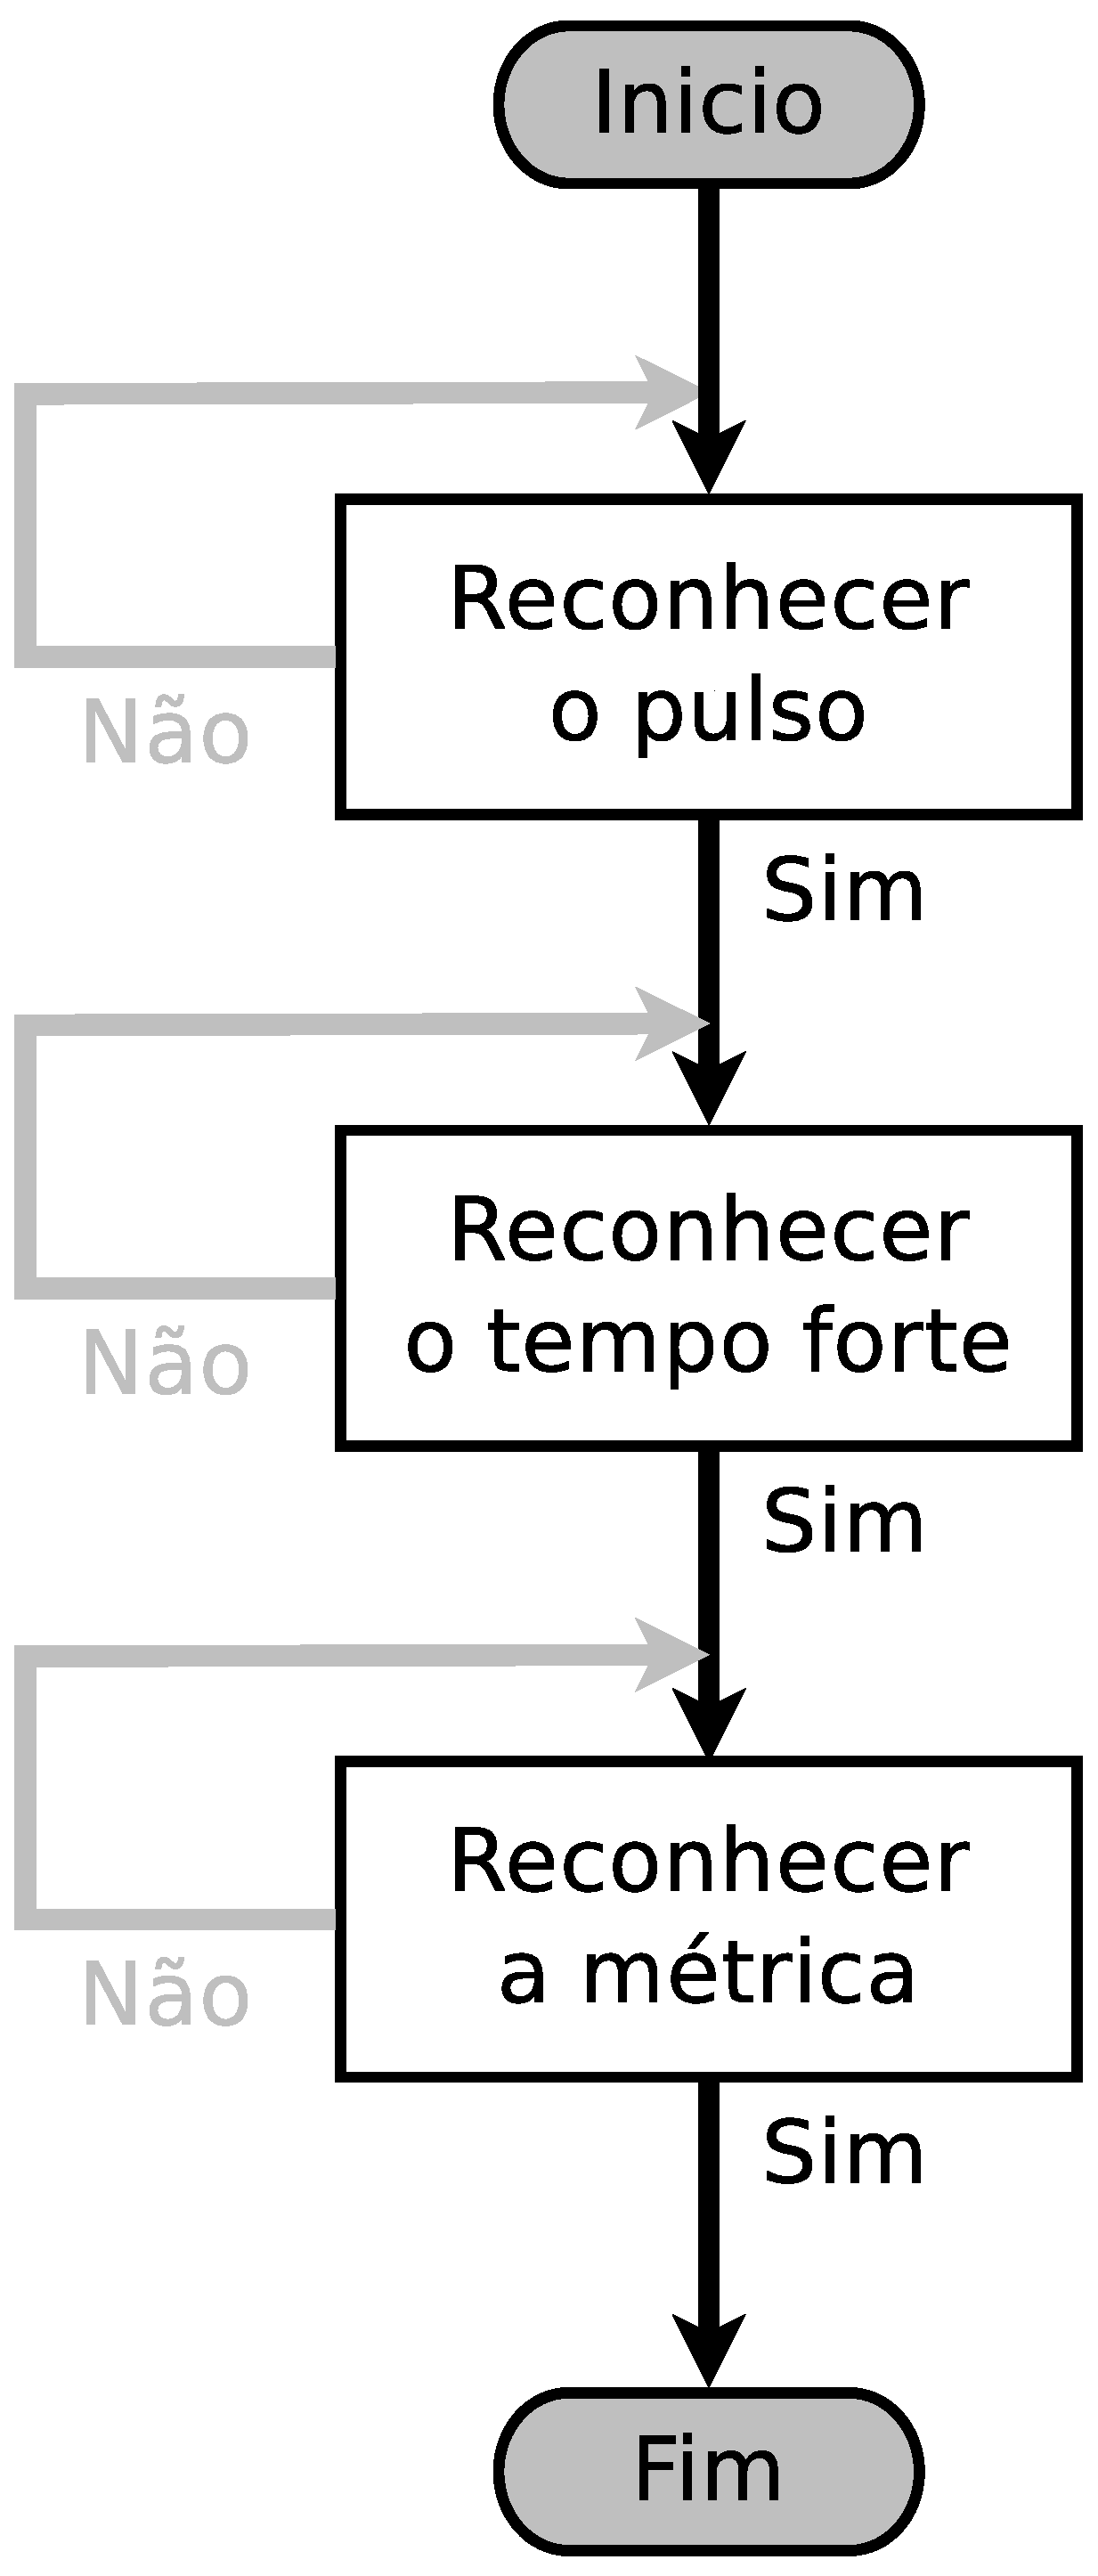
\includegraphics[width=0.6\textwidth]{chapters/cap-musica-musicalidade/dancanopulso1.eps}
\caption{Percebendo a métrica método 1.}
\label{fig:fluxodancanopulso1}
\end{subfigure}
~%
\begin{subfigure}[c]{0.45\textwidth}
\centering 
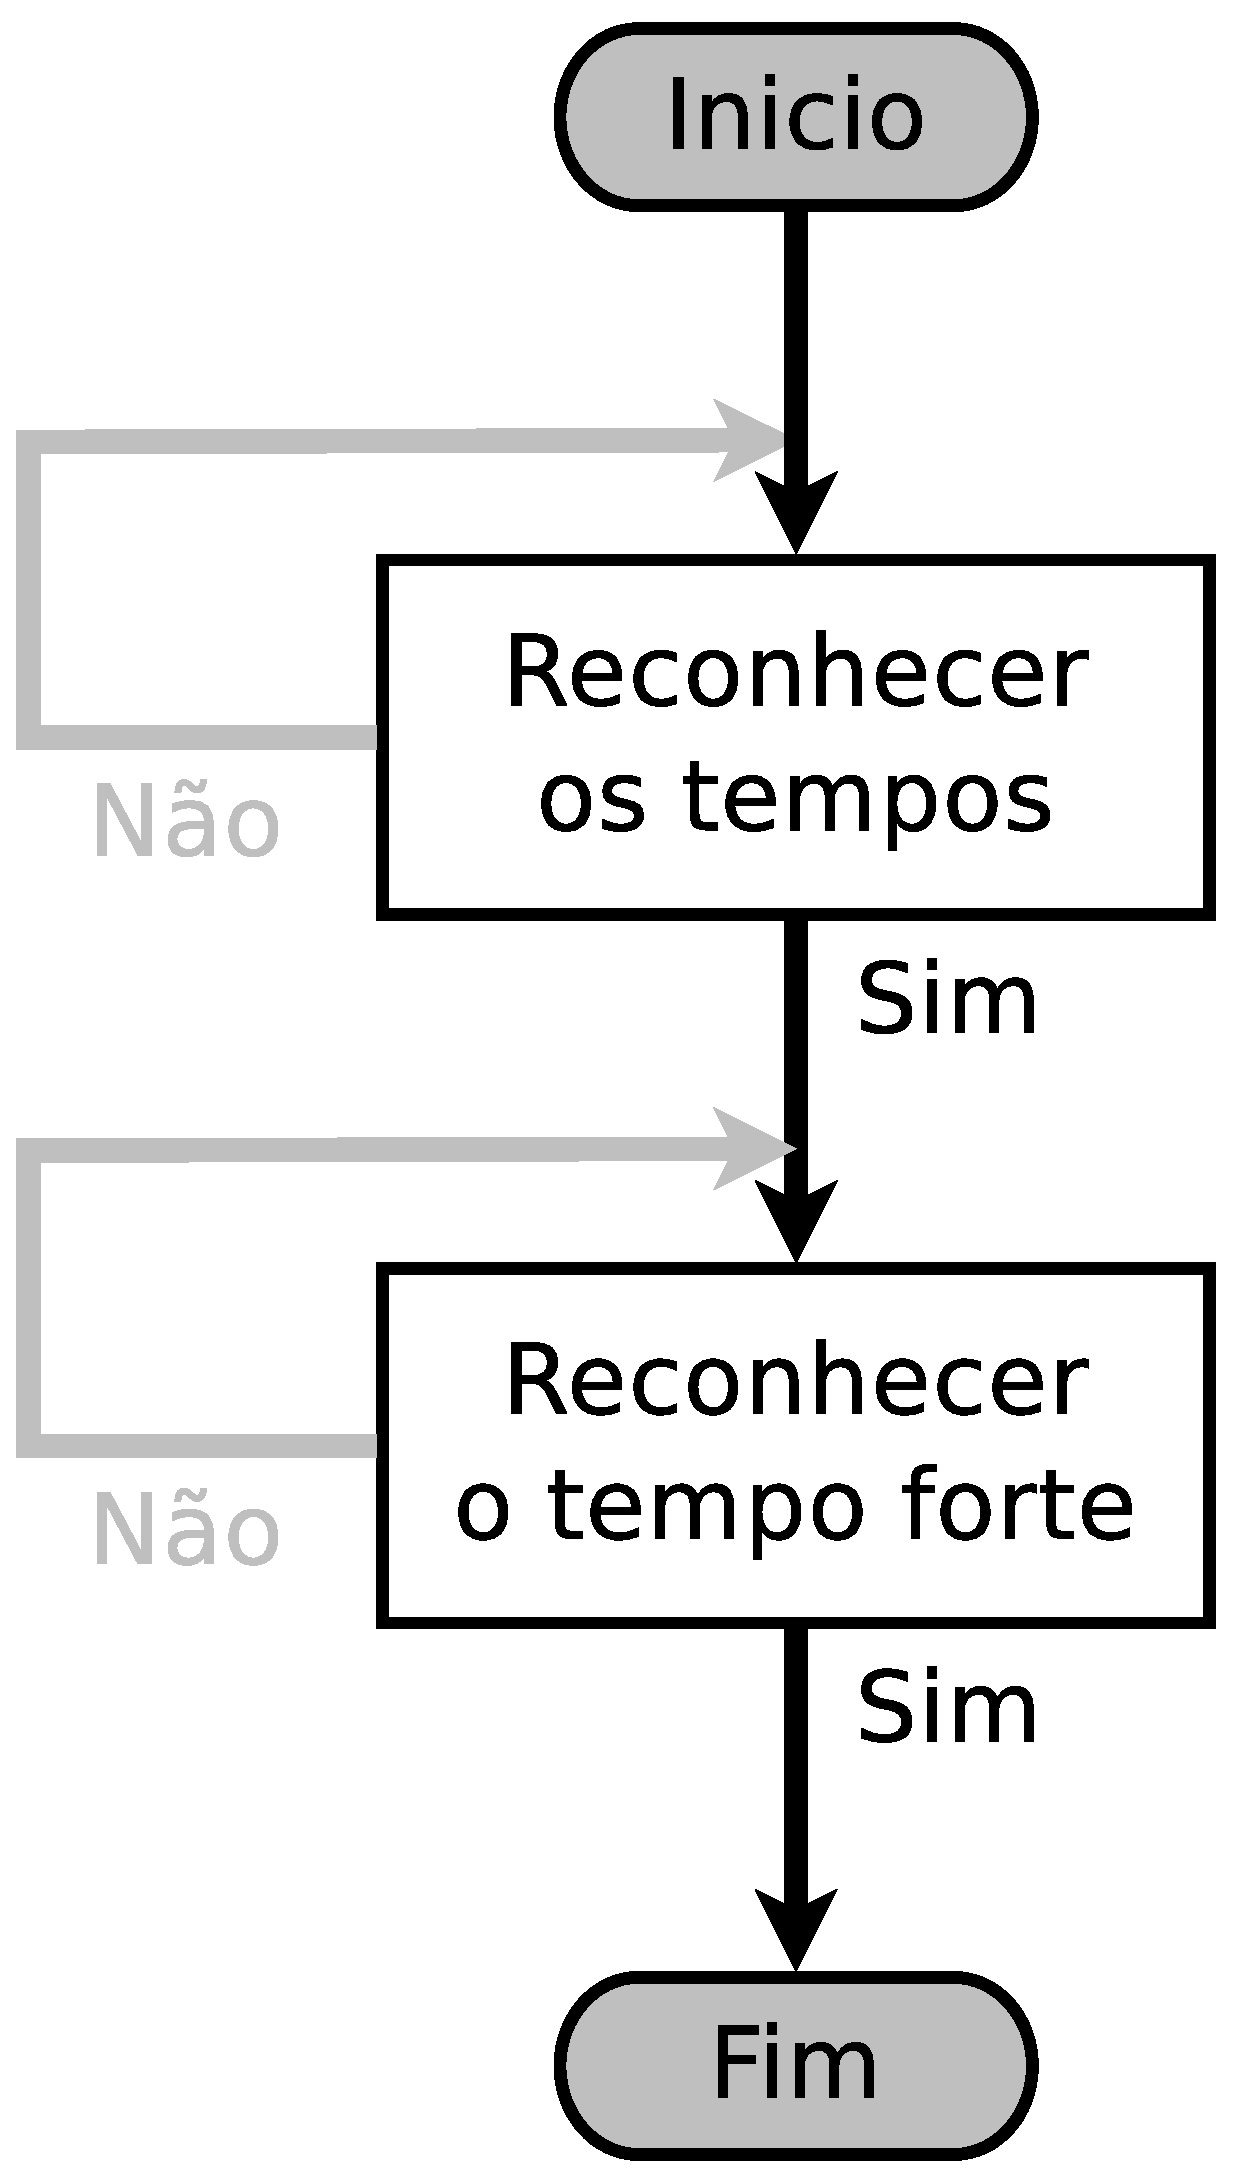
\includegraphics[width=0.6\textwidth]{chapters/cap-musica-musicalidade/dancanopulso2.eps}
\caption{Percebendo a métrica método 2}
\label{fig:fluxodancanopulso2}
\end{subfigure}
    \caption{Percebendo métrica}\label{fig:fluxodancanopulso}
\end{figure}


%%%%%%%%%%%%%%%%%%%%%%%%%%%%%%%%%%%%%%%%%%%%%%%%%%%%%%%%%%%%%%%%%%%%%%%%%%%%%%%%
%%%%%%%%%%%%%%%%%%%%%%%%%%%%%%%%%%%%%%%%%%%%%%%%%%%%%%%%%%%%%%%%%%%%%%%%%%%%%%%%
\section{\textcolor{blue}{Percepção rítmica da percussão no samba}}
\index{Musicalidade!Percepção rítmica}
\label{sec:percepcaoouvinte}
Quando escutamos uma música, na qual é tipicamente dançado samba de gafieira,
podemos distinguir que a soma dos sonidos produzidos pelos instrumentos realizam 
um padrão de repetição muito particular, geralmente ligado as onomatopeias: ``tchic-tchic tum'' ou ``tum tum''.


A Figura \ref{fig:abc-caquarela} representa os compassos 18, 19 e 20 da  
composição musical ``Aquarela do Brasil'' escrita
por Ary Barroso em 1939 \cite{AquarelaDoBrasil}; 
a versão mostrada na figura teve arranjos por Irineu Krüger \cite{Irineu}. 
Nesta versão, a música está representada com 1 voz ou coro de voces (``Voice Choir'') e 4 
instrumentos (``Eb'',``Bb'',``Strings'' e ``D. Bass''), que usam uma 
formula de compasso $2/4$, de modo que cada compasso
é binário e
pode ser preenchido usando duas semínimas (2\quarternote).
\begin{figure}[ht]
\centering
%\includegraphics[width=\textwidth]{chapters/cap-fundamentos/aquarela.png}
\begin{abc}[name=abc-caquarela]
% abcm2ps aquarela.abc  -O aquarela.ps
% ps2epsi aquarela.ps aquarela.eps
%
X: 1 % start of header
T: Brazil - Aquarela do Brasil
C: Music: Ary Barroso, 1939
C: Arranged by: Irineu Krüger
K: C % scale: C major
M: 2/4 % formula do compasso
%
V:1 clef=treble name="Voice Choir" sname="Voice Choir"
V:2 clef=treble name="Eb" sname="Eb"
V:3 clef=treble name="Bb" sname="Bb"
V:4 clef=treble name="Strings" sname="Strings"
V:5 clef=bass   name="D. Bass" sname=""D. Bass"
%
%
[V:1] "18" C'3/2A/2C2  |"19" A3/2(G/2 G/2)E1E/2  |"20" z/2 C'1A/2 C'1C'1  |
w:    Ó Bras-sil        sam-ba_ que dá       bam-bo-leio_ 
w:    Ó Bras-sil        ver-de que dá_       pa-ra~o mun-do 
%
%
[V:2] G1z/2G1z/2G1  | G1z/2G1z/2G1  | G1z/2G1z/2G1  |
%
%
[V:3] z4  | z4  | z4  |
%
%
[V:4] G1z/2G1z/2G1  | G1z/2G1z/2G1  | G1z/2G1z/2G1  |
%
%
[V:5] C,2 G,,2  | C,1 z1 G,,2  | C,2 G,,2  |
\end{abc}
\caption{3 compassos da partitura da composição ``Aquarela do brasil''}
\label{fig:abc-caquarela}
\end{figure}

\subsection{Percepção do: tchic-tchic tum}
Analisando este fragmento de partitura e escutando a música produzida, 
podemos perceber que os instrumentos executados em conjunto geram um sonido identificável
com a onomatopeia ``tchic-tchic tum''.
Assim, o inicio de cada compasso coincide com o ``tum''; 
sendo que este é o momento em que a maioria dos instrumentos produzem um sonido, 
de modo que a sensação para o ouvinte é de uma potencia sonora maior. 
Cada instrumento prolongará seu sonido de forma diferente; 
porem,  podemos dizer que: o ``tum'' ocupa $1$ tempo (\quarternote), 
e que o sonido de um ``tchic'' ocupa médio tempo (0.5\quarternote),
sendo que o primeiro ``tchic'' é executado no tempo fraco de ``D. Bass'', 
e o segundo ``tchic'' solapa e obscurece ao  primeiro, 
que é executado na parte fraca do tempo fraco de ``Strings'' ou ``Eb'' (fazendo um contratempo);
conseguindo assim criar a ilusão do ``tchic-tchic tum'', com ``tchic''s de médio tempo ; de modo que:
\begin{equation}
tchic + tchic = tum ~~ \Longleftrightarrow ~~ tchic = \frac{tum}{2}.
\end{equation}
 
Por outro lado, se a percepção do ouvinte é mais
aguçada, poderá escutar ``a tchic-tchic tum''; 
neste caso, o sonido ``tum'' é solapado por o sonido de ``a'',
quando transcorrido um $75\%$ do primeiro tempo do compasso; 
o sonido ``a''  se prolonga incluindo a parte forte do tempo fraco subsequente, 
este sonido é executado pelos instrumentos ``Eb'' e ``Strings'' e constitui uma sincopa \cite[pp. 143]{medteoria}.


Pelo exposto anteriormente, agora podemos simplificar a partitura para gerar um sonido com onomatopeia
``tchic-tchic tum'', como é mostrado na Figura \ref{fig:abc-contratempo1}.
Assim,
o instrumento 1 executa dois sonidos, de modo que o primeiro contribui ao sonido 
``tum'' e o segundo sonido gera o segundo ``tchic'' do compasso; por outro lado,
o instrumento 2 executa um ritmo com um padrão
de repetição de dois sonidos ``tum'' e ``tchic'', nesse ordem;
sendo que a nota executada no tempo forte produz um sonido mais agudo que a 
executada no tempo fraco, isto é assim para poder diferenciar melhor ambos tempos.
\begin{figure}[ht]
\centering
\begin{abc}[name=abc-contratempo1,width=0.6\linewidth]
X: 1 % start of header
K: C % scale: C major
M:2/4
%T: Contratempo num compasso binário
V:1 clef=treble name="Instrumento 1" sname="Inst. 1"
V:2 clef=bass   name="Instrumento 2" sname="Inst. 2"
[V:1] |: " ""T/2"G1 " ""T/2"z1 " ""T/2"z1 " ""T/2"G1 | " ""T/2"G1 " ""T/2"z1 " ""T/2"z1 " ""T/2"G1  :|
w:    tum                tchic                       tum                   tchic           
[V:2] |:  "Tempo"C,2 "Tempo"G,,2  | "Tempo"C,2 "Tempo"G,,2  :|
w:    tum       tchic              tum       tchic            
\end{abc}
\caption{Padrão de repetição para gerar um sonido de onomatopeia ``tchic tchic tum''.}
\label{fig:abc-contratempo1}
\end{figure}

Conhecido tudo isto, é fácil perceber como existe uma diferencia, entre 
o que percebemos ao escutar uma música, e a forma como esta é escrita na partitura;
pois como é visto na Figura \ref{fig:abc-contratempo1}, quando escrevemos
um sonido com um padrão de repetição na ordem ``tum tchic-tchic'', para o ouvinte é mais natural associar
este sonido com o padrão ``tchic-tchic~tum'', devido a que \textbf{quando um ser humano fala, este usa a pausa
para denotar o final de uma palavra}. Da mesma forma, ao escutar uma música, traduzimos
que o sonido que tem um silencio maior apos ser executado marca o final do ciclo
do padrão de repetição. Assim, o que o músico vê ao ler a partitura
é um padrão de repetição ``tum tchic-tchic'', sendo que  um
ouvinte interpretará de forma instintiva que o padrão é ``tchic-tchic tum''.

\subsection{\textcolor{red}{Percepção do: tum~tum}}

Analisando o fragmento de partitura, na Figura \ref{fig:abc-caquarela}, 
e tentando isolar o instrumento ``D. Bass'',
podemos perceber que este gera um sonido identificável com a onomatopeia ``tum tum''.
Podemos ver isoladamente este instrumento, na Figura \ref{fig:abc-contratempo1tumtum}.
\begin{figure}[ht]
\centering
\begin{abc}[name=abc-contratempo1tumtum,width=0.5\linewidth]
X: 1 % start of header
K: C % scale: C major
M:2/4
%T: Contratempo num compasso binário
V:1 clef=bass   name="D. Bass" sname="D. Bass"      
[V:1] |: "Tempo"C,2 "Tempo"G,,2  | "Tempo"C,2 "Tempo"G,,2  :|
w:    tum       tum         tum       tum            
\end{abc}
\caption{Padrão de repetição para gerar um sonido de onomatopeia ``tum tum''.}
\label{fig:abc-contratempo1tumtum}
\end{figure}

%%%%%%%%%%%%%%%%%%%%%%%%%%%%%%%%%%%%%%%%%%%%%%%%%%%%%%%%%%%%%%%%%%%%%%%%%%%%%%%%
%%%%%%%%%%%%%%%%%%%%%%%%%%%%%%%%%%%%%%%%%%%%%%%%%%%%%%%%%%%%%%%%%%%%%%%%%%%%%%%%
\section{\textcolor{blue}{Treinamentos de percepção rítmica}}
\index{Musicalidade!Percepção rítmica}
Nestos exercícios um equipamento ou um professor, 
deve executar uma vez as seguintes sequencias rítmicas, e
seguidamente os ouvintes ou estudantes devem repetir o sonido, 
incluindo as acentuações, primeiro com palmas e logo com os pés.
Nos seguintes exemplos é escrito com maiúscula a onomatopeia 
com acento musical, para lembrar este detalhe na execução do som. 

Percepção do ritmo (TUM tum), a tempo, na Figura \ref{fig:abc-percepcionritmica1}.
\begin{figure}[H]
\centering
\begin{abc}[name=abc-percepcionritmica1,width=0.4\linewidth]
X: 1 % start of header
K: C stafflines=1 % scale: C major
M: 2/4 %meter - compasso
%Q:1/4=80
V:1 clef=perc stem=up %name="Pauta com clave de fá"   sname="Pauta com clave de fá"
[V:1] |: B2  B2| B2  B2 :|  
w: TUM tum TUM tum         
\end{abc}
\caption{Treinamento de percepção rítmica a tempo.}
\label{fig:abc-percepcionritmica1}
\end{figure}

Percepção do ritmo (tum TUM), a contratempo, na Figura \ref{fig:abc-percepcionritmica2}.
\begin{figure}[H]
\centering
\begin{abc}[name=abc-percepcionritmica2,width=0.4\linewidth]
X: 1 % start of header
K: C stafflines=1 % scale: C major
M: 2/4 %meter - compasso
%Q:1/4=80
V:1 clef=perc stem=up %name="Pauta com clave de fá"   sname="Pauta com clave de fá"
[V:1] |: B2  !>!B2| B2  !>!B2 :|
w:      tum  TUM tum TUM   
\end{abc}
\caption{Treinamento de percepção rítmica a contratempo.}
\label{fig:abc-percepcionritmica2}
\end{figure}


Percepção do ritmo (TUM tchic-tchic), a tempo, na Figura \ref{fig:abc-percepcionritmica3}.
\begin{figure}[H]
\centering
\begin{abc}[name=abc-percepcionritmica3,width=0.5\linewidth]
X: 1 % start of header
K: C stafflines=1 % scale: C major
M: 2/4 %meter - compasso
%Q:1/4=80
V:1 clef=perc stem=up %name="Pauta com clave de fá"   sname="Pauta com clave de fá"
[V:1] |: B2  B1 B1| B2  B1 B1 :|
w: TUM tchic tchic TUM tchic tchic      
\end{abc}
\caption{Treinamento de percepção rítmica a tempo.}
\label{fig:abc-percepcionritmica3}
\end{figure}

Percepção do ritmo (tum TCHIC-tchic), a contratempo, na Figura \ref{fig:abc-percepcionritmica4}.
\begin{figure}[H]
\centering
\begin{abc}[name=abc-percepcionritmica4,width=0.5\linewidth]
X: 1 % start of header
K: C stafflines=1 % scale: C major
M: 2/4 %meter - compasso
%Q:1/4=80
V:1 clef=perc stem=up %name="Pauta com clave de fá"   sname="Pauta com clave de fá"
[V:1] |: B2  !>!B1 B1| B2  !>!B1 B1 :|
w: tum TCHIC tchic tum TCHIC tchic         
\end{abc}
\caption{Treinamento de percepção rítmica a contratempo.}
\label{fig:abc-percepcionritmica4}
\end{figure}


Percepção do ritmo (TUM tum-e), a tempo, na Figura \ref{fig:abc-percepcionritmica5}.
\begin{figure}[H]
\centering
\begin{abc}[name=abc-percepcionritmica5,width=0.5\linewidth]
X: 1 % start of header
K: C stafflines=1 % scale: C major
M: 2/4 %meter - compasso
%Q:1/4=80
V:1 clef=perc stem=up %name="Pauta com clave de fá"   sname="Pauta com clave de fá"
[V:1] |: B2  B3/2 B1/2| B2  B3/2 B1/2 :|
w: TUM tum e TUM tum e 
\end{abc}
\caption{Treinamento de percepção rítmica a tempo.}
\label{fig:abc-percepcionritmica5}
\end{figure}

Percepção do ritmo (tum TUM-e), a contratempo, na Figura \ref{fig:abc-percepcionritmica6}.
\begin{figure}[H]
\centering
\begin{abc}[name=abc-percepcionritmica6,width=0.5\linewidth]
X: 1 % start of header
K: C stafflines=1 % scale: C major
M: 2/4 %meter - compasso
%Q:1/4=80
V:1 clef=perc stem=up %name="Pauta com clave de fá"   sname="Pauta com clave de fá"
[V:1] |: B2  !>!B3/2 B1/2| B2  !>!B3/2 B1/2 :| 
w: tum TUM e tum TUM e 
\end{abc}
\caption{Treinamento de percepção rítmica a contratempo.}
\label{fig:abc-percepcionritmica6}
\end{figure}

Percepção do ritmo (TUM tum-e TUM~tchic-tchic), a tempo, na Figura \ref{fig:abc-percepcionritmica7}.
\begin{figure}[H]
\centering
\begin{abc}[name=abc-percepcionritmica7,width=0.45\linewidth]
X: 1 % start of header
K: C stafflines=1 % scale: C major
M: 2/4 %meter - compasso
%Q:1/4=80
V:1 clef=perc stem=up %name="Pauta com clave de fá"   sname="Pauta com clave de fá"
[V:1] |: B2  B3/2 B1/2| B2  B1 B1  :| 
w: TUM tum e TUM tchic tchic   
\end{abc}
\caption{Treinamento de percepção rítmica a tempo.}
\label{fig:abc-percepcionritmica7}
\end{figure}

%%%%%%%%%%%%%%%%%%%%%%%%%%%%%%%%%%%%%%%%%%%%%%%%%%%%%%%%%%%%%%%%%%%%%%%%%%%%%%%%
%%%%%%%%%%%%%%%%%%%%%%%%%%%%%%%%%%%%%%%%%%%%%%%%%%%%%%%%%%%%%%%%%%%%%%%%%%%%%%%%
\section{\textcolor{green}{Contagem de tempos correográficos}}
\index{Musicalidade!Tempos coreográficos}

falar da possibilidade de contar 123 567 sim se usa um nome diferente a contagem de tempo musical,
exemplo, tempos coreográficos

Ver Figura \ref{fig:contagemtempocoreografico}.
\begin{sidewaysfigure}
    \centering
    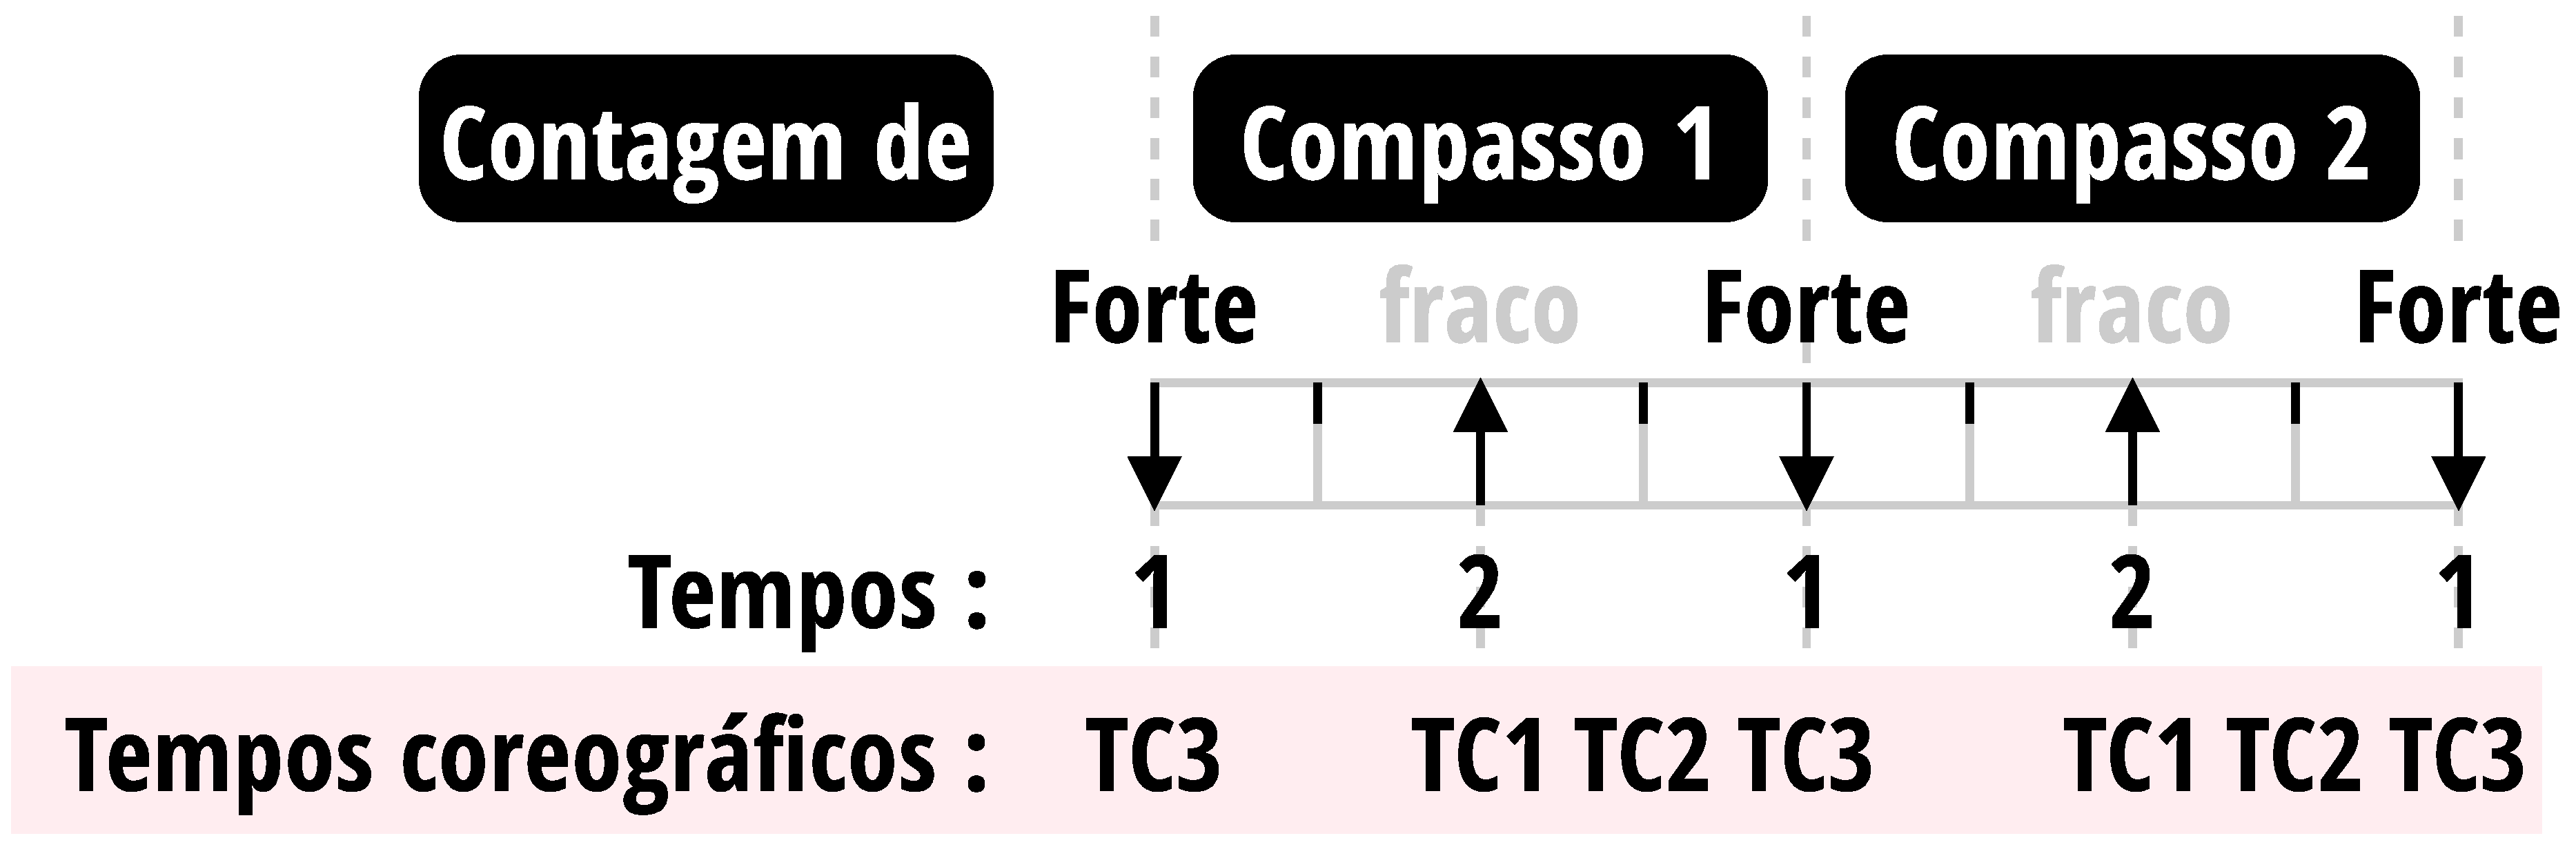
\includegraphics[width=\textwidth]{chapters/cap-musica-musicalidade/contagemtempocoreografico.eps}
    \caption{Contando tempos coreograficos.}
    \label{fig:contagemtempocoreografico}
\end{sidewaysfigure}

%%%%%%%%%%%%%%%%%%%%%%%%%%%%%%%%%%%%%%%%%%%%%%%%%%%%%%%%%%%%%%%%%%%%%%%%%%%%%%%%
%%%%%%%%%%%%%%%%%%%%%%%%%%%%%%%%%%%%%%%%%%%%%%%%%%%%%%%%%%%%%%%%%%%%%%%%%%%%%%%%
\section{\textcolor{green}{Contagens dos passos para o ensino}}
Antes de iniciar esta seção é importante mencionar uma
problemática que é vista com muita frequência nas escolas de dança; 
esta é gerada devido a que: A forma em que os tempos são contados 
na música, é
diferente à realizada entre profissionais da música e da dança. 
Sendo que a contagem dos profissionais da música segue a \hyperref[def:Metrica]{\textbf{métrica}} indicada na partitura,
e no caso de profissionais da dança segue geralmente um enfoque 
particular a cada escola de dança, visando só em muitos casos o fácil entendimento do aluno da
execução do movimento programado para essa aula, e não uma rigorosidade teórica no uso de termos e 
expressões musicais.




\subsection{Contagem de 3 passos em 2 tempos}
Esta diferença na forma de perceber o inicio e o final do ciclo de repetição,
vista na Seção \ref{sec:percepcaoouvinte}, 
leva a um problema quando se quer ser rigoroso na forma de contar os tempos nos compassos; 
por exemplo, na Tabela \ref{tab:ritmo1} 
podemos ver 4 formas distintas, que podem adotar as pessoas, 
para contar os tempos nos compassos indicando a distribuição de tempos, 
onde ``$T$'' representa um tempo do compasso.
\begin{table}[ht]
  \centering
  \begin{tabular}    {c|ccc|c}
    \hline
    Tipos de contagem       & $T/2$ & $T/2$   & $T$ (Forte) & Recomendável?\\
    \hline
    Contagem 1: & tchic  & tchic  & tum   & Sim\\
    Contagem 2: & 2     & e     & 1     & Sim\\ \hline
    Contagem 3: & Con   & tra  & Tempo & Não\\
    Contagem 4: & 1     & e     & 2     & Não\\  \hline
    Contagem 5: & 1     & 2     & 3     & Depende\\ \hline
    \hline
  \end{tabular}
  \caption{Tipos de contagem na samba de gafieira.}
\label{tab:ritmo1}
\end{table}

As formas de contagem que recomendo são:
\begin{itemize}
\item \textbf{A contagem 1}, 
devido que a principio, pode ser usada sem aprofundar demasiado 
na notação musical, de modo que só precisa ser explicado que a duração de um 
``tum'' é o dobro que um ``tchic'', e anexar que tipicamente veremos que o ``tum''
acontece no tempo 1 do compasso; 
%de modo que outra contagem valida seria ``tum tchic tchic''; 
porem, a contagem 1 não está restrita ao uso destas silabas (``tchic'' e ``tum''), 
em geral esta contagem representa a quase qualquer padrão de repetição
que use duas silabas diferentes, como por exemplo os padrões: ``ta-ta kum'', ``tic-tic kum'', etc. 
Este tipo de contagem já é muito usada na pratica e na literatura, pois 
podemos achar variantes como ``quick-quick slow'' (rápido-rápido lento no idioma inglês)
ou ``tic-tic tum'' seguindo a notação usada por Perna no seu livro sobre samba de gafieira \cite[pp. 146]{perna2002samba}.
\item \textbf{A contagem 2}, segue a notação de tempos na partitura, este tipo de
contagem é coerente com a musica, porem precisa de uma major explicação, 
para pessoas não iniciadas na musica e a dança. Porem, isto não quer dizer que seu
entendimento seja complexo, e sim que precisa um investimento em horas de aula
um pouco major que a contagem 1.
Mesmo assim, devemos ter cuidado pois pode-se dar o caso que a partitura não tenha compassos binários 
e sim quaternários, com contagens ``2 e 3'' ``4 e 1'', 
criando este tipo de contagem mais caminhos onde podemos perder coerência com a contagem na partitura.\\
\end{itemize}


Entre as contagens que não recomendo estão:
\begin{itemize}
\item \textbf{A contagem 3} (``con-tra tempo''), 
devido a que o uso deste padrão pode confundir às pessoas que desconhecem 
a definição formal do termo contratempo \cite[pp. 16]{mascarenhascurso} \cite[pp. 36]{azevedocompor}, 
e levar a confusão de achar que um contratempo é só uma distribuição de 3 tempos, 
sendo um o dobro dos outros dois, em termos de tempos execução.
\item \textbf{A contagem 4} é não recomendada, devido a que como é visto nas Figuras 
\ref{fig:abc-caquarela} e \ref{fig:abc-contratempo1}, musicalmente a contagem estaria invertida,
dado que tipicamente o ``tum'' se execute no tempo 1.\\
\end{itemize}

Finalmente, a contagem que precisa um cuidado especial:
\begin{itemize}

\item \textbf{A contagem 5} precisa ser bem explicada, 
devido a que não segue as notações musicais; porem, seu uso pode ser resgatado,
se fazemos em todo instante uma aclaração, que se trata de ``tempos coreográficos''.
Assim, ficara claro para o estudante, que estes não correspondem necessariamente, 
com os tempos musicais que também devem ser ensinados.

%não é recomendada, 
%por motivos similares aos apresentados para a contagem 4. 
%Além do fato que os números atribuídos estão distantes da
%notação verdadeira na partitura, mesmo sim esta houvesse sido escrita num compasso quaternário.
\end{itemize}

\subsection{\textcolor{red}{Contagem de 2 passos em 2 tempos}}


Tabela \ref{tab:ritmoconta2}

\begin{table}[ht]
  \centering
  \begin{tabular}    {c|cc|c}
    \hline
    Tipos de contagem       & $T$ (fraco)  & $T$ (Forte)& Recomendável?\\
    \hline
    Contagem 1: & tum  & TUM  & Sim\\
    Contagem 2: & 2     & 1     & Sim\\
    Contagem 3: & tempo & Tempo & Sim\\ \hline
    Contagem 4: & 1     & 2     & Não\\ \hline
    Contagem 5: & 1     & 3     & Depende\\  \hline
    \hline
  \end{tabular}
  \caption{Tipos de contagem na samba de gafieira.}
\label{tab:ritmoconta2}
\end{table}

%%%%%%%%%%%%%%%%%%%%%%%%%%%%%%%%%%%%%%%%%%%%%%%%%%%%%%%%%%%%%%%%%%%%%%%%%%%%%%%%
%%%%%%%%%%%%%%%%%%%%%%%%%%%%%%%%%%%%%%%%%%%%%%%%%%%%%%%%%%%%%%%%%%%%%%%%%%%%%%%%
\section{\textcolor{red}{Procurando um bom ``Timing''}}
\index{Musicalidade!Timing}
Procurando o momento certo

 sincronização 
 %[https://www.infopedia.pt/dicionarios/ingles-portugues/timing]

 sentido de oportunidade 
 %[https://www.infopedia.pt/dicionarios/ingles-portugues/timing]


%%%%%%%%%%%%%%%%%%%%%%%%%%%%%%%%%%%%%%%%%%%%%%%%%%%%%%%%%%%%%%%%%%%%%%%%%%%%%%%%
%%%%%%%%%%%%%%%%%%%%%%%%%%%%%%%%%%%%%%%%%%%%%%%%%%%%%%%%%%%%%%%%%%%%%%%%%%%%%%%%
\section{\textcolor{red}{Dançando no tempo e em contratempo}}
\index{Musicalidade!Dançando no tempo}
\index{Musicalidade!Dançando em contratempo}


Que significa dançar no tempo forte? 
pisar o tum  no tempo forte.

Se percebo que estou pisando no fraco como corrigir?
podemos usar
\begin{itemize}
\item Caminhada em contratempo
\item Fazemos balaços um número impar de vezes.
\end{itemize}


A Figura \ref{fig:tempovscontratempo}.

\begin{figure}[h]
    \centering 
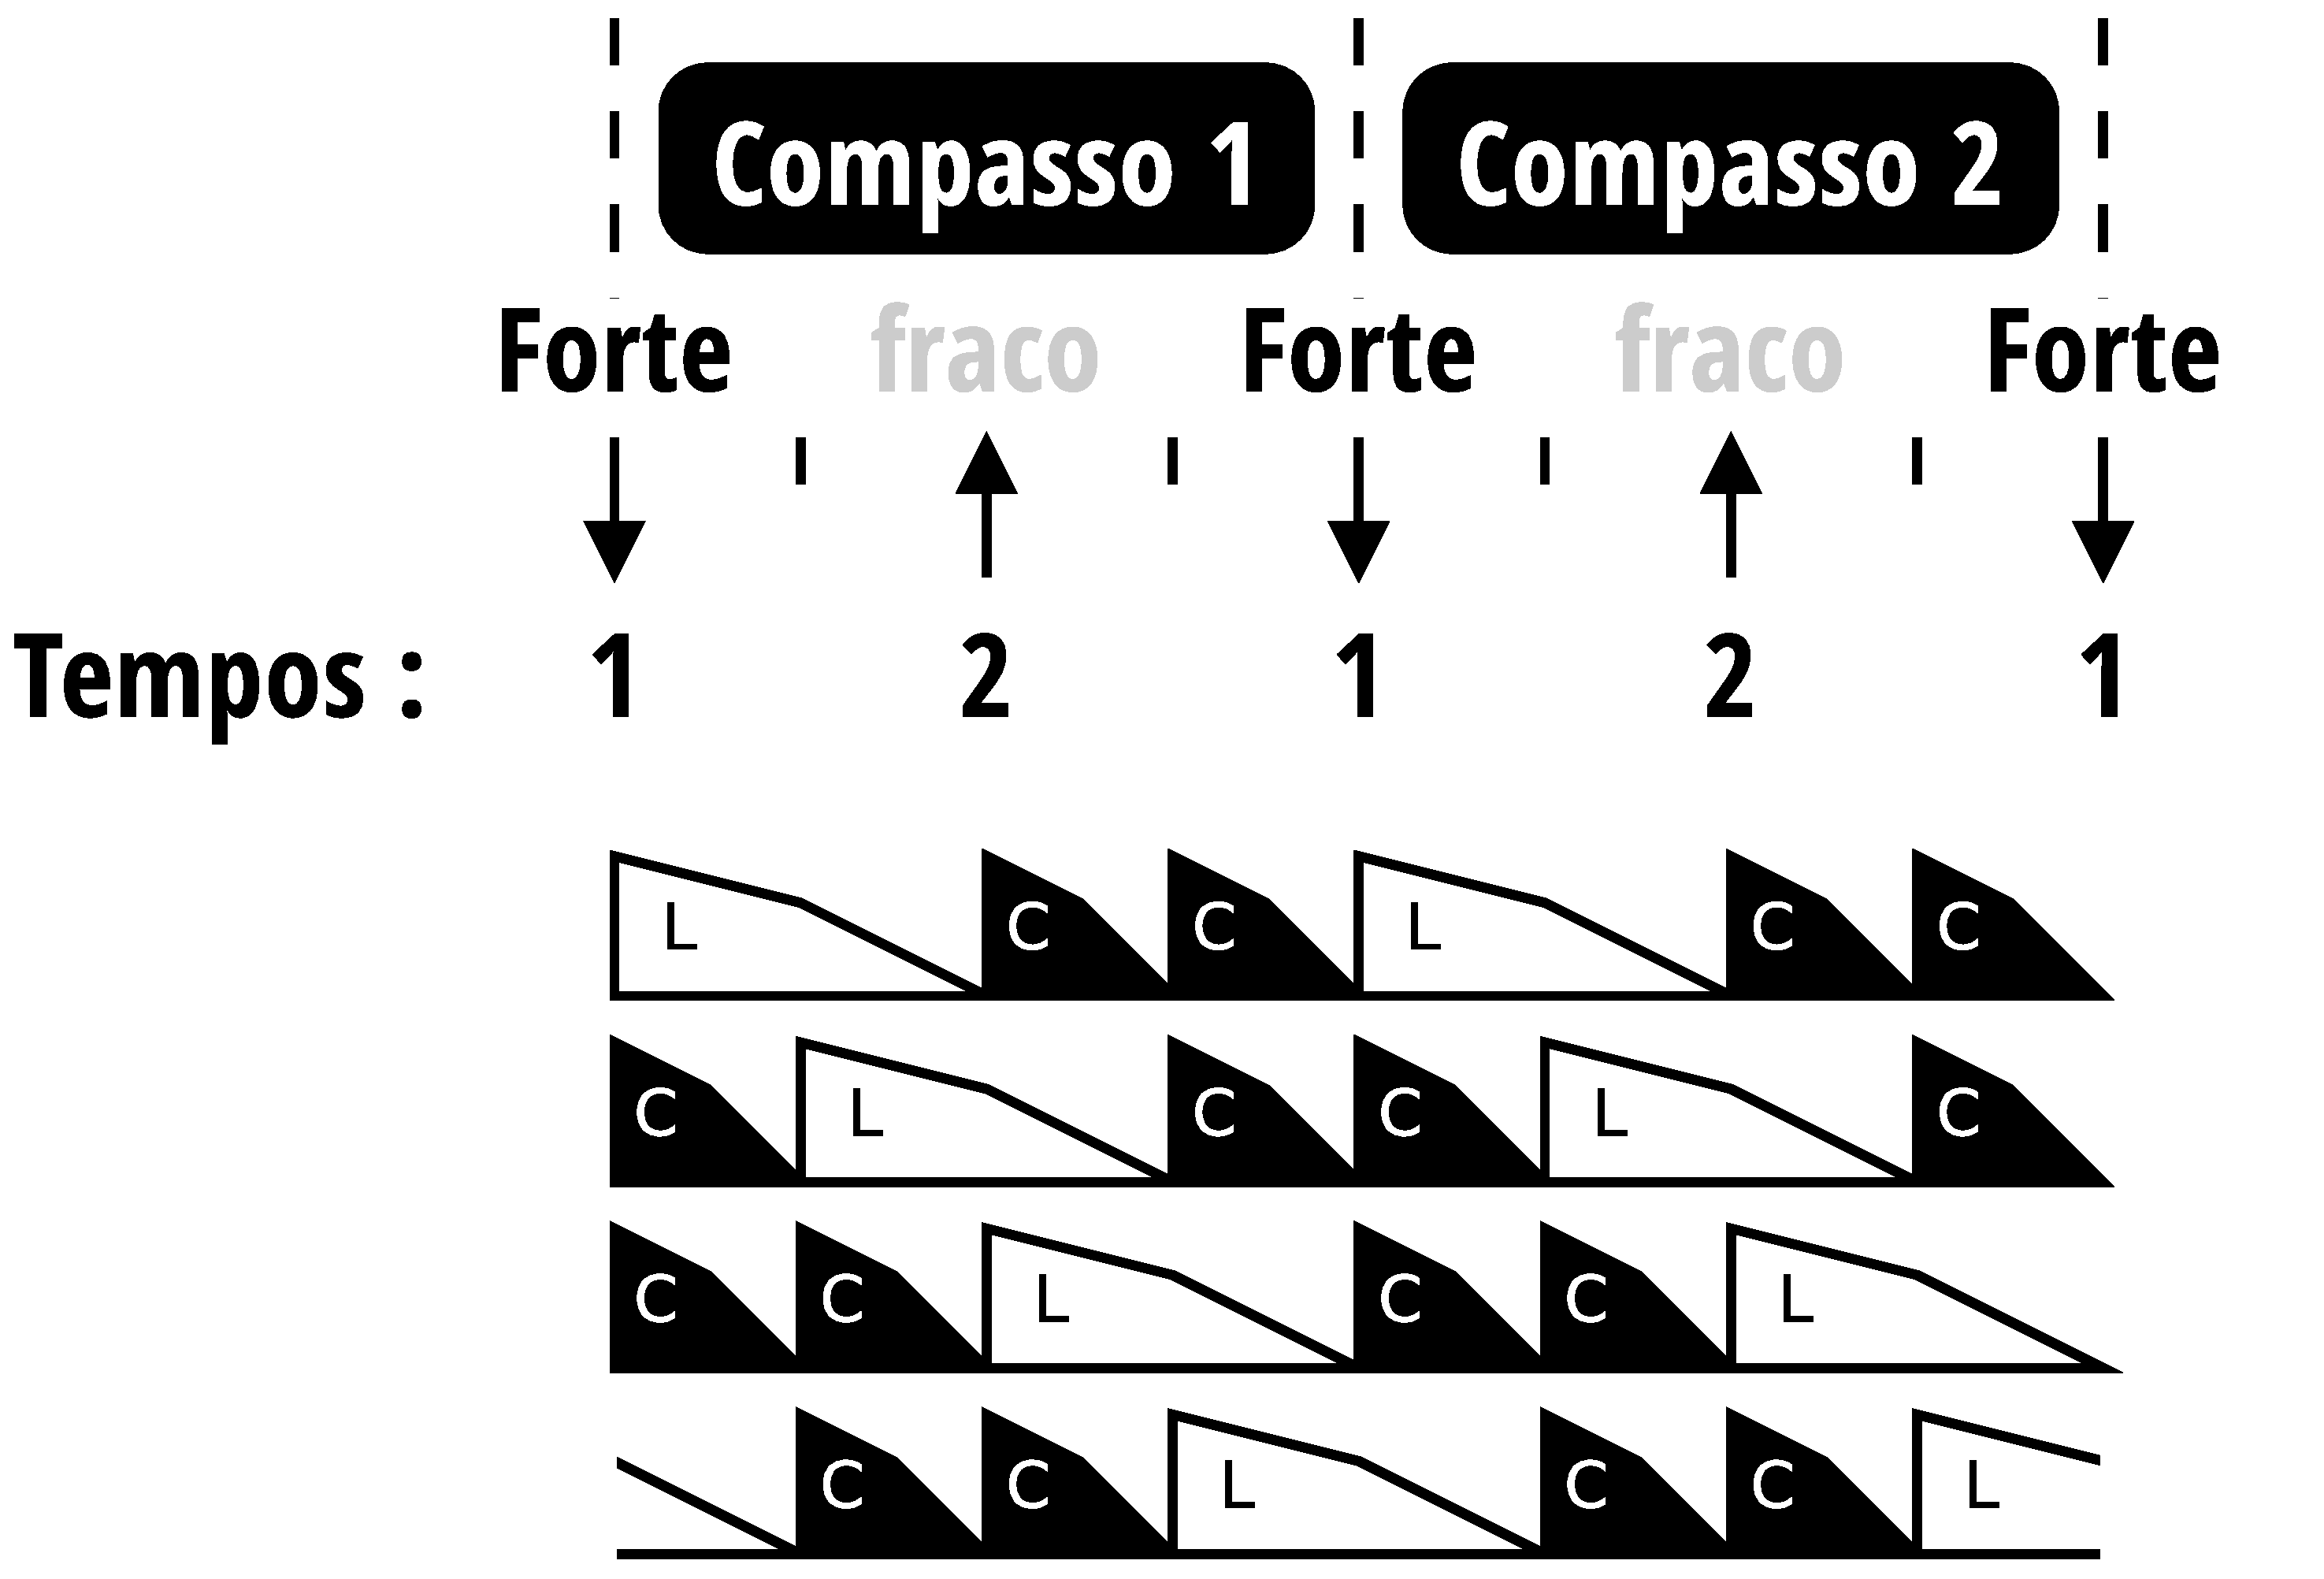
\includegraphics[width=0.9\textwidth]{chapters/cap-musica-musicalidade/bailarcontratempo.eps}
    \caption{Percebendo métrica}\label{fig:tempovscontratempo}
\end{figure}


%%%%%%%%%%%%%%%%%%%%%%%%%%%%%%%%%%%%%%%%%%%%%%%%%%%%%%%%%%%%%%%%%%%%%%%%%%%%%%%%
%%%%%%%%%%%%%%%%%%%%%%%%%%%%%%%%%%%%%%%%%%%%%%%%%%%%%%%%%%%%%%%%%%%%%%%%%%%%%%%%
\section{\textcolor{red}{Percebendo frases musicais}}
\index{Musicalidade!Frase musical}
Porque é importante reconhecer as frases com final conclusivo e suspensivo,
\begin{itemize}
\item Si tentamos dançar no tempo forte, conhecer a existência de ambos tipos de final de frase, 
no ajuda a ter certeza que estamos indo bem com o tempo, e que não somos nos que erramos achando o tempo forte,
e sim, que existe mais de um tipo de final de frase, e que este foi diferente, foi suspensivo.
E não nos deixaremos enganar por finais suspensivos sincopados (que parecem conclusivos),
e estaremos mais seguros de nossa dança.
\item Uma vez temos ciência da existência de ambos tipos de final, 
podemos usar suas particularidades. Por exemplo,
uma frase com final conclusivo indica o fim, literal, de uma ideia musical, 
pelo que si desejamos ter coerência com a música, 
nosso movimento e parada deve demostrar a mesma resolução,
e dar a ideia de que o relato de nossa dança acabou de expressar uma ideia completa;
para isto podemos fazer um movimento explosivo com pausa abrupta, 
ou agregar uma posse final, ou tao simples como um abraço elegante com ponto final.
Por outro lado, se o final de frase musical é suspensivo, 
a ideia transmitida tem uma sensação de pergunta,
ou de uma resposta meditativa que se apaga aos poucos e pede uma reflexão ao ouvinte,
em outras palavras um assunto não completamente  concluído.
Nesse sentido, se nosso objetivo é ter uma coerência com a música,
o relato que expressa nossa dança deve dar essa sensação de uma ideia que se apaga aos poucos,
ou de pergunta; por exemplo, isto se consegue dando um passo final em tempo forte,
seguido de movimentos corporais no lugar ate a ultima nota musical.
\end{itemize}

Exemplo de final conclusivo e suspensivo na Figura \ref{fig:conclusivo-suspensivo1}. 

\begin{figure}[H]
\centering
\begin{abc}[name=abc-conclusivo-suspensivo1]
X: 1 % start of header
K: C stafflines=1 % scale: C major
M: 2/4 %meter - compasso
L:1/8
Q:1/4=80
V:1 clef=perc stem=up %name="Pauta com clave de fá"   sname="Pauta com clave de fá"
[V:1] |:B3/2 B/2 B1 B1| B/2  B2 z/2  z1 | B3/2 B/2 B1 B1| B2 z2:|
w:      TA!  ti-ta-ta   TI!-ta             TA!  ti-ta-ta  TA!
\end{abc}
\caption{Frase de 8 tempos.}
\label{fig:conclusivo-suspensivo1}
\end{figure}



\subsection{\textcolor{red}{percebendo frases com final conclusivo}}
% Breaks (frases com final conclusivo):
% Moreira Da Silva - Idade Não é Documento - https://www.youtube.com/watch?v=-mwwkz3TwxU
% JOGANDO COM O CAPETA MOREIRA DA SILVA - https://www.youtube.com/watch?v=MYngGP43lkY
% ??? Moreira Da Silva - Na Subida Do Morro - https://www.youtube.com/watch?v=fD8Hh4CFPkk

\subsection{\textcolor{red}{percebendo frases com final suspensivo}}

% Breaks (Voz: frases final conclusivo + suspensivo + contratempo)
% https://www.youtube.com/watch?v=ujEDJhBx2W0
% Breaks (voz: frases final conclusivo + suspensivo):
% https://www.youtube.com/watch?v=YC9nVbVrUHU

\subsubsection{\textcolor{red}{percebendo frases com final suspensivo a contratempo e sincopado}}
% Breaks (voz: frases final suspensivo + sincopado):
% Eu Sou A Marrom - https://www.youtube.com/watch?v=QMUkDngZmjo

%%%%%%%%%%%%%%%%%%%%%%%%%%%%%%%%%%%%%%%%%%%%%%%%%%%%%%%%%%%%%%%%%%%%%%%%%%%%%%%%
%%%%%%%%%%%%%%%%%%%%%%%%%%%%%%%%%%%%%%%%%%%%%%%%%%%%%%%%%%%%%%%%%%%%%%%%%%%%%%%%
\section{\textcolor{red}{Contando e medindo a frase musical}}
\index{Musicalidade!Frase musical}
Provavelmente 4
\begin{itemize}
\item 4 compassos
\item 8 compassos
\item 2 compassos
\item 16 compassos
\end{itemize}


Ver Figura \ref{fig:contagemtemposfrase}.
\begin{sidewaysfigure}
    \centering
    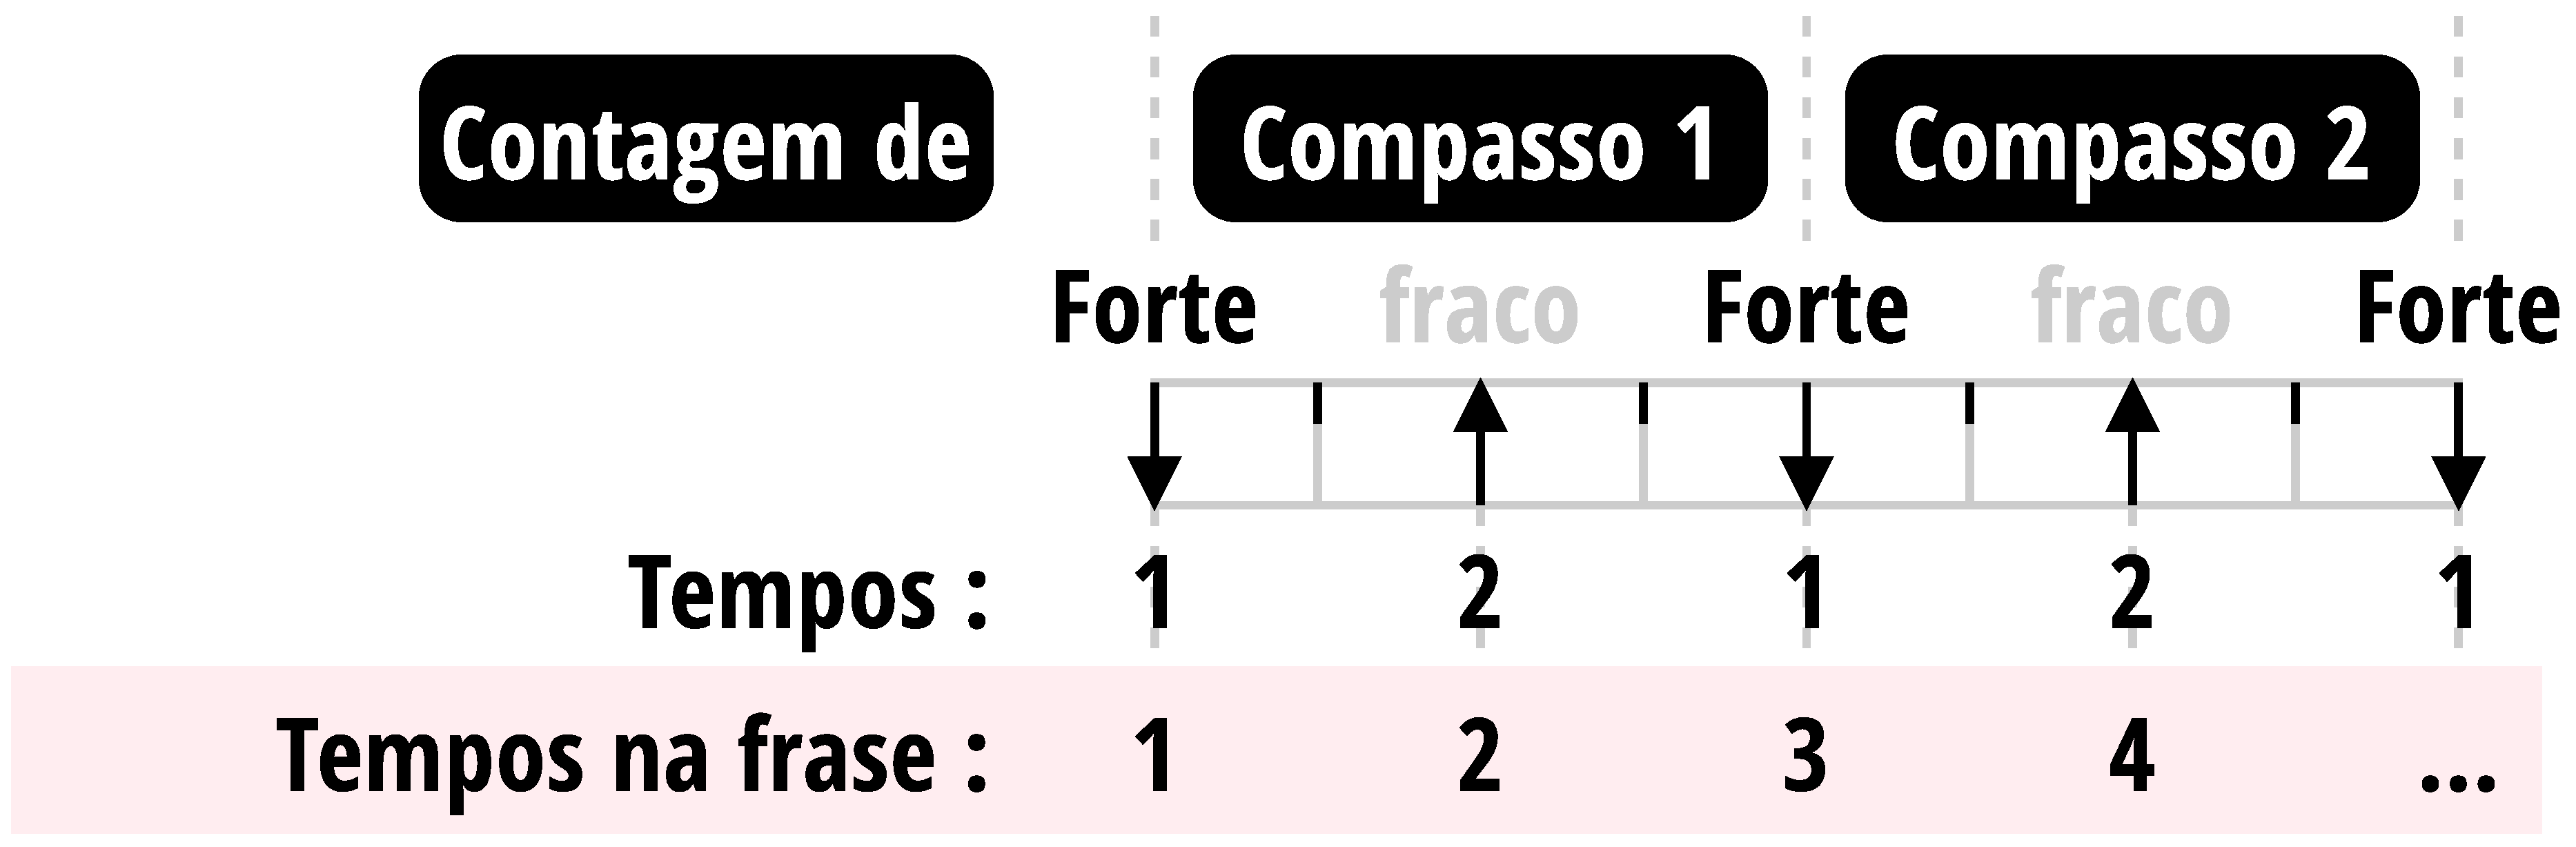
\includegraphics[width=\textwidth]{chapters/cap-musica-musicalidade/contagemtemposfrase.eps}
    \caption{Contando a frase musical.}
    \label{fig:contagemtemposfrase}
\end{sidewaysfigure}

%%%%%%%%%%%%%%%%%%%%%%%%%%%%%%%%%%%%%%%%%%%%%%%%%%%%%%%%%%%%%%%%%%%%%%%%%%%%%%%%
%%%%%%%%%%%%%%%%%%%%%%%%%%%%%%%%%%%%%%%%%%%%%%%%%%%%%%%%%%%%%%%%%%%%%%%%%%%%%%%%
\section{\textcolor{red}{Percebendo e usando o ``break'' da música}}
\index{Musicalidade!Breques ou paradas}


%%%%%%%%%%%%%%%%%%%%%%%%%%%%%%%%%%%%%%%%%%%%%%%%%%%%%%%%%%%%%%%%%%%%%%%%%%%%%%%%
%%%%%%%%%%%%%%%%%%%%%%%%%%%%%%%%%%%%%%%%%%%%%%%%%%%%%%%%%%%%%%%%%%%%%%%%%%%%%%%%
\section{\textcolor{red}{Aspectos da musicalidade na dança}}
\subsection{\textcolor{red}{Dançar no pulso}}
Ver Figura \ref{fig:lamentoconsolopulso1}.
\begin{sidewaysfigure}
    \centering
    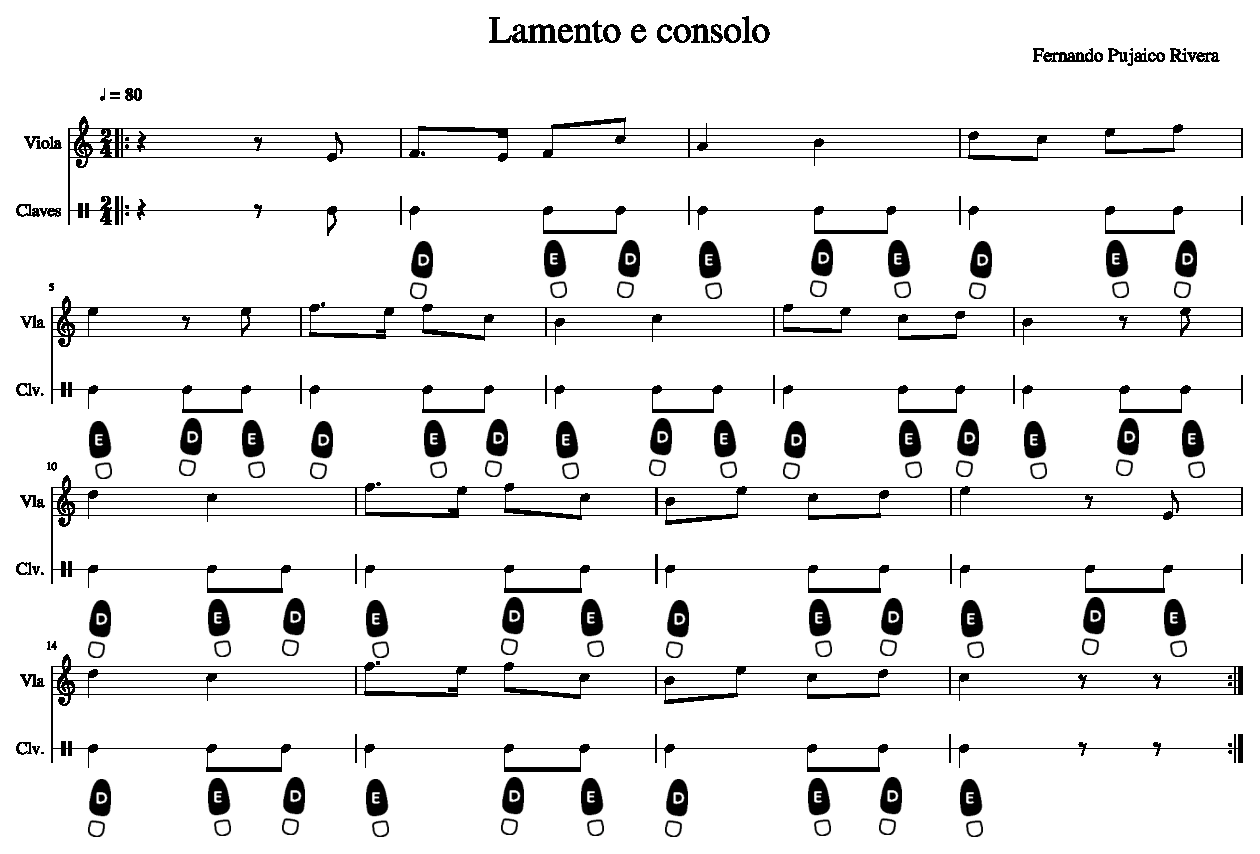
\includegraphics[width=\textwidth]{chapters/cap-musica-musicalidade/lamento-e-consolo-clave-pulso-1.eps}
    \caption{Música dançada no pulso.}
    \label{fig:lamentoconsolopulso1}
\end{sidewaysfigure}

Ver Figura \ref{fig:lamentoconsolopulsobreak1}.
\begin{sidewaysfigure}
    \centering
    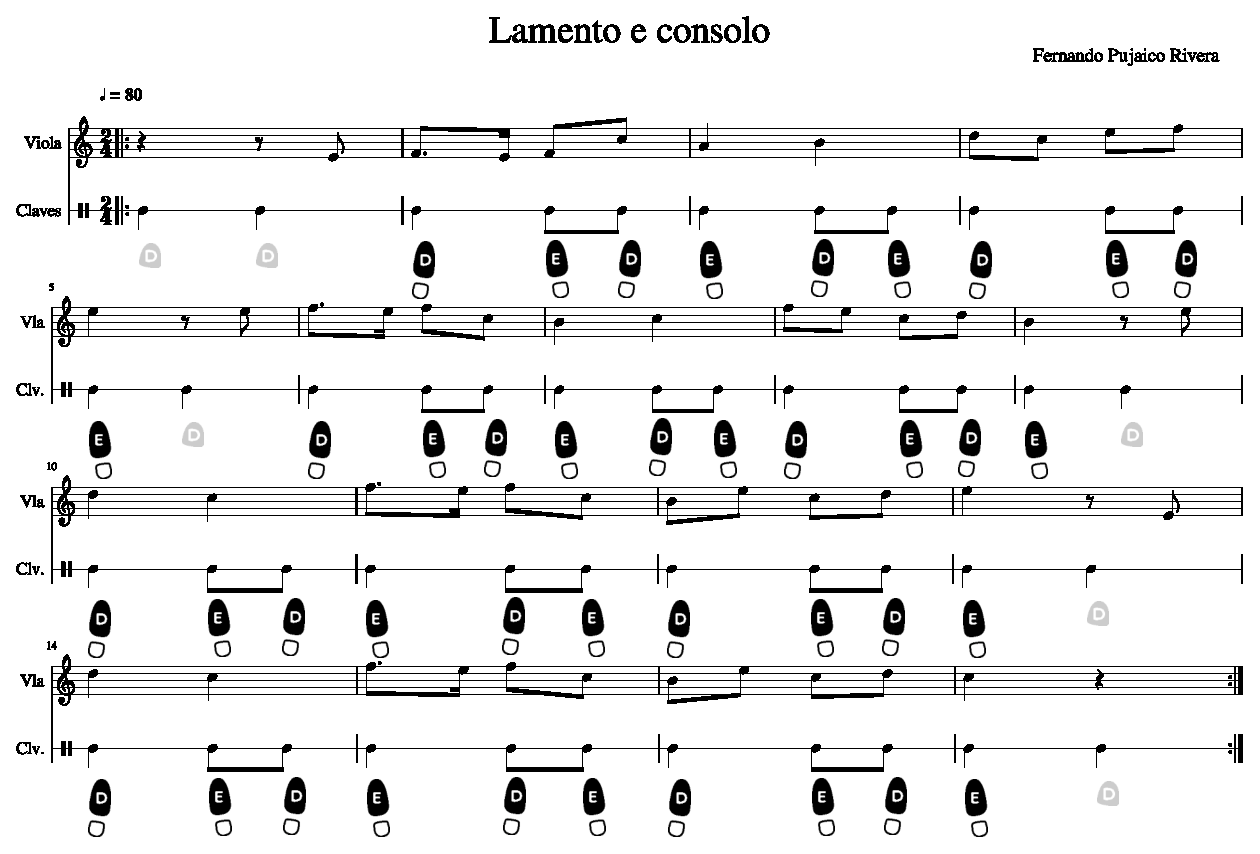
\includegraphics[width=\textwidth]{chapters/cap-musica-musicalidade/lamento-e-consolo-clave-pulso+break-1.eps}
    \caption{Música dançada no pulso e usando breaks.}
    \label{fig:lamentoconsolopulsobreak1}
\end{sidewaysfigure}


\subsection{\textcolor{red}{Dançar no ritmo}}
Una buena regla general, especialmente si es nuevo en el baile, es mantener el pulso o el ritmo en su cuerpo.

Mantener el pulso o el ritmo en la cabeza o en el pecho es una de las cosas más fáciles para cualquier persona.

%https://tangowords.wordpress.com/2017/01/10/elements-of-musicality-beat-and-rhythm/
\begin{comment}
quando começamos a dançar, aprendemos a dançar com o batida, 
depois de um tempo começamos a dançar com o ritmo, eventualmente descobrimos como dançar com a música. 
Claro, estes não são separados; Quando dançamos ao ritmo, 
também dançamos ao  batida. 
E quando dançamos a música, os elementos de batida e ritmo também estão lá.

Ao falar com os dançarinos, acho que às vezes há confusão entre batida e ritmo. 
Simplificando, a batida é o pulso constante que você sente na melodia, 
como um tique-taque do relógio. É com o que você pode bater palmas ou bater o pé em. 
O ritmo é o padrão real que as notas de comprimentos diferentes fazem, 
que em uma música podem ser as mesmas que os padrões de palavras. 
Além do tamanho das notas, o ritmo também é criado quando algumas notas são enfatizadas sobre outras.

Geralmente, a dance music (exceto valsa / vals, claro) tem quatro batidas no bar. 
As batidas 1 e 3 são as batidas fortes (o compás no tango) as batidas 2 e 4 
são as batidas fracas (às vezes chamadas de batidas de costas ou de batidas). 
Em seu nível mais simples, quando dançamos, tendemos a pisar nas batidas 1 e 3. 
(Embora, ao bater palmas, a preferência seja aplaudir a batida de trás).

Claro, tudo isso se aplica a qualquer dança criativa de parceiros, 
não apenas ao tango. Em algumas aulas, às vezes você ouve: 
"Este é um movimento de seis batidas" ou "Este é um movimento de doze batidas". 
Isso só é verdade se você estiver se limitando a dançar mecanicamente e unicamente 
ao batida da música. Se você está dançando ao ritmo, 
quantas batidas levará dependendo de como você trabalha com a música.

É muito fácil cair na armadilha de pensar em padrões de passos e se tornar um 
"dançarino de um e três". (E, infelizmente, a batida fortemente acentuada de boa 
parte do que se passa por dance music tende a encorajar isso ... mas isso é outra 
história para outro post no blog!) Somos dançarinos, não metrônomos.
\end{comment}

Ver Figura \ref{fig:lamentoconsoloritmo1}.
\begin{sidewaysfigure}
    \centering
    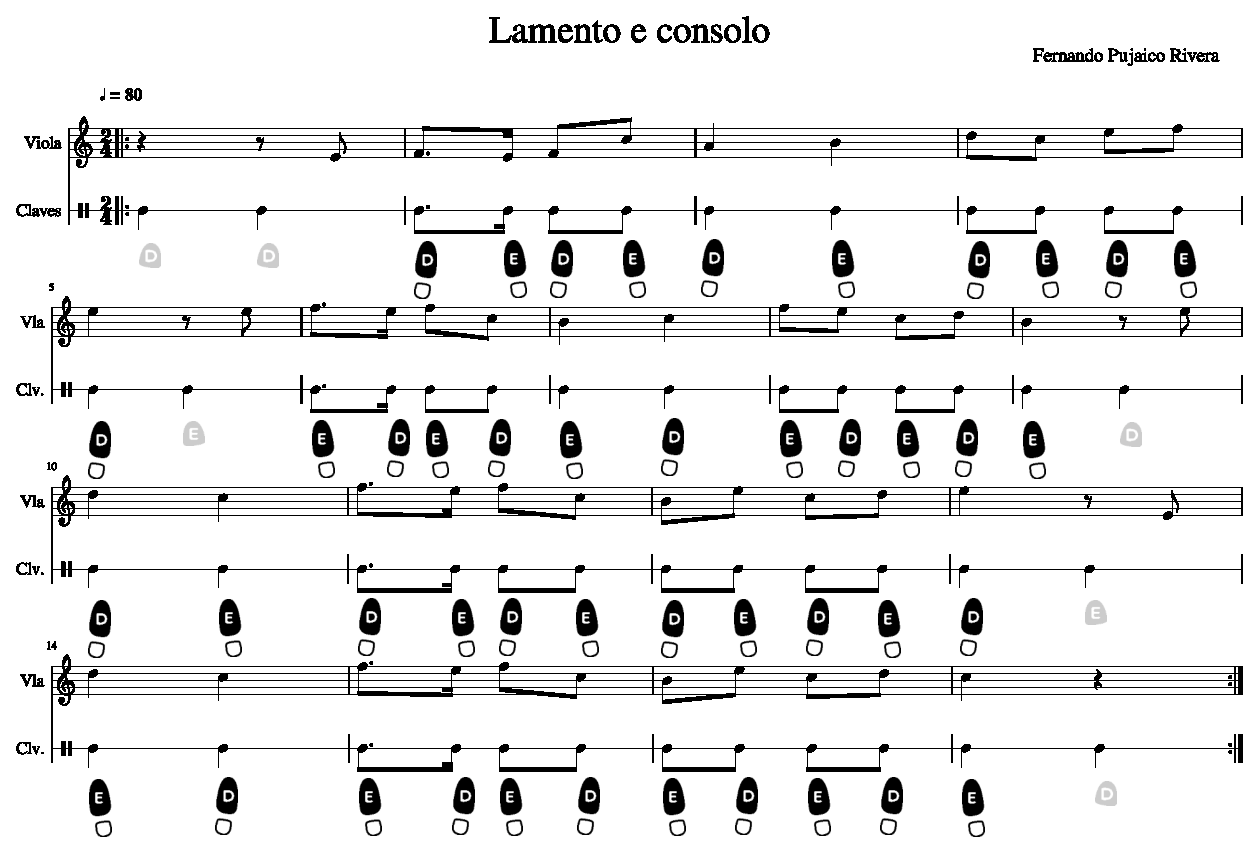
\includegraphics[width=\textwidth]{chapters/cap-musica-musicalidade/lamento-e-consolo-clave-ritmo-1.eps}
    \caption{Música dançada no ritmo.}
    \label{fig:lamentoconsoloritmo1}
\end{sidewaysfigure}

\subsection{\textcolor{red}{Dançar na melodia}}
Para darle un poco más de libertad y creatividad, mantener el pulso o el ritmo en sus pies le brinda la capacidad de interpretar la melodía con el resto de su cuerpo, si así lo desea.

\subsection{\textcolor{red}{Dançar na música}}

%%%%%%%%%%%%%%%%%%%%%%%%%%%%%%%%%%%%%%%%%%%%%%%%%%%%%%%%%%%%%%%%%%%%%%%%%%%%%%%%
%%%%%%%%%%%%%%%%%%%%%%%%%%%%%%%%%%%%%%%%%%%%%%%%%%%%%%%%%%%%%%%%%%%%%%%%%%%%%%%%
\section{\textcolor{red}{Mickey mousing}}
\index{Musicalidade!Mickey mousing}
onomatopeia andante


%%%%%%%%%%%%%%%%%%%%%%%%%%%%%%%%%%%%%%%%%%%%%%%%%%%%%%%%%%%%%%%%%%%%%%%%%%%%%%%%
%%%%%%%%%%%%%%%%%%%%%%%%%%%%%%%%%%%%%%%%%%%%%%%%%%%%%%%%%%%%%%%%%%%%%%%%%%%%%%%%
\section{\textcolor{red}{Leitmotif}}
\index{Musicalidade!Leitmotif}
motivo principal \cite[pp. 7]{bribitzer2015understanding} \cite[pp. 465]{apel1969harvard}

%%%%%%%%%%%%%%%%%%%%%%%%%%%%%%%%%%%%%%%%%%%%%%%%%%%%%%%%%%%%%%%%%%%%%%%%%%%%%%%%
%%%%%%%%%%%%%%%%%%%%%%%%%%%%%%%%%%%%%%%%%%%%%%%%%%%%%%%%%%%%%%%%%%%%%%%%%%%%%%%%
\section{\textcolor{red}{Seguindo isoladamente os instrumentos}}
Seria uma forma de mickey mousing
\begin{itemize}
\item Dançando choro-chorinho no ritmo esquecendo o ``Tchic-Tchic Tum''.
\item Trabalhando com marionetas um em cada mão, ou dedo.
\item Cada aluno simula que tem um instrumento virtual e toca ele.
\end{itemize}

%%%%%%%%%%%%%%%%%%%%%%%%%%%%%%%%%%%%%%%%%%%%%%%%%%%%%%%%%%%%%%%%%%%%%%%%%%%%%%%%
%%%%%%%%%%%%%%%%%%%%%%%%%%%%%%%%%%%%%%%%%%%%%%%%%%%%%%%%%%%%%%%%%%%%%%%%%%%%%%%%
\section{\textcolor{red}{Embolada, Rap e musicalizar poesias}}
\index{Musicalidade!Frase musical}
% https://scielo.conicyt.cl/scielo.php?script=sci_arttext&pid=S0719-32622018000100030
Figura \ref{rap:emocional-protesto1}

\begin{figure}[H]
\centering
\begin{abc}[name=abc-emocional-protesto1]
X: 1 % start of header
K: C stafflines=1 % scale: C major
M: 2/4 %meter - compasso
Q:1/4=100
V:1 clef=perc stem=up %name="Pauta com clave de fá"   sname="Pauta com clave de fá"
[V:1] |:!>!B3/2 B/2 B1 B1| B3/2 B/2 B1 B1 | B2 B2| B2 B1 B1:|
\end{abc}
\caption{Frase de 8 tempos, com palavra final grave.}
\label{rap:emocional-protesto1}
\end{figure}


\begin{citando}
Vida simples, metáfora de um corpo;\\
luzes cobertas, as lágrimas expostas.\\
Vida simples, luta contra o tempo;\\
brilha, existe, e terás respostas.\\
\end{citando}


Tabela \ref{tab:verso1}

\begin{table}[h!]
\begin{center}
\begin{tabular}{|l||l||l||l|} % 
\hline
compasso 1 & compasso 2   & compasso 3   & compasso 4 \\ \hline \hline
\textbf{Vi}da       & \textbf{sim}ples, me- & \textbf{tá}fora de um  & \textbf{cor}po;  \\ \hline
\textbf{lu}zes  co- & \textbf{ber}tas, as   & \textbf{lá}grimas ex-  & \textbf{pos}tas. \\ \hline
\textbf{Vi}da       & \textbf{sim}ples,     & \textbf{lu}ta contra o & \textbf{tem}po;  \\ \hline
\textbf{bri}lha, e- & \textbf{xis}te,       & \textbf{e} terás res-  & \textbf{pos}tas. \\ \hline
\end{tabular}
\caption{Verso 1.}
\label{tab:verso1}
\end{center}
\end{table}


Figura \ref{rap:emocional-protesto2}

\begin{figure}[H]
\centering
\begin{abc}[name=abc-emocional-protesto2]
X: 1 % start of header
K: C stafflines=1 % scale: C major
M: 2/4 %meter - compasso
Q:1/4=100
V:1 clef=perc stem=up %name="Pauta com clave de fá"   sname="Pauta com clave de fá"
[V:1] |:!>!B3/2 B/2 B1 B1| B3/2 B/2 B1 B1 | B2 B2| B2 z2:|
\end{abc}
\caption{Frase de 8 tempos, com palavra final aguda.}
\label{rap:emocional-protesto2}
\end{figure}

%%%%%%%%%%%%%%%%%%%%%%%%%%%%%%%%%%%%%%%%%%%%%%%%%%%%%%%%%%%%%%%%%%%%%%%%%%%%%%%%
%%%%%%%%%%%%%%%%%%%%%%%%%%%%%%%%%%%%%%%%%%%%%%%%%%%%%%%%%%%%%%%%%%%%%%%%%%%%%%%%
\section{\textcolor{red}{Texturas vs. Articulação na dança }}
\index{Musicalidade!Articulação}
Articulação das notas musicais refletido na nossa dança

Legato vs. sttacato

%https://blog.steezy.co/what-are-textures-in-dancing/
%https://www.elevateartsuk.co.uk/what-are-textures-dynamics-in-dance-and-how-can-i-use-them/


